\chapter{データ実験の詳細}
\label{chap:data}
\section{使用したモデルの詳細}
第3章で述べたとおり使用した対戦データは弱いAIを先番とし,強いAIを後手としている.
AIの強さは一手ごとの探索を行う時間(time),付録Cで述べる$C_{puct}$,ニューラルネットワークの訓練段階におけるエポック数の値によって調整した.
timeと$C_{puct}$,エポック数はいずれも値が大きい程モデルは強くなると考えられる.(エポック数については付録\ref{chap:baseline}を参照)
対戦データ生成時のパラメータは表\ref{table:param-battle}の幅からゲームごとにランダムな値を採用した.
これはパラメータの値を変化させることでゲームデータに多様性を持たせるためである.
\begin{table}[H]
	\caption{対戦データのパラメータ}
	\label{table:param-battle}
	\centering
	\scalebox{0.98}[0.98]{
		\begin{tabular}{c|c|c}
			モデル&強&弱\\ \hline
			time    & 3-5 & 0-2 \\ 
			$C_{puct}$ & 0.8-1   & 0-0.5 \\
			エポック数 & 200 & 1 \\

		\end{tabular}
	}
	\label{table:battle}
\end{table}

\section{対戦結果の詳細}
2000ゲームのうち1983ゲームは強いAI(後番)の勝利となった.
また,ゲームごとの手数は75\%のゲームが36手以内で終了している.
そのため,データ実験ではゲームの中盤と言える13$\sim$24手目のデータを使用した.
図\ref{fig:stepCum}にゲームの終了手数の累計グラフを示す.
\begin{figure}[t]
	\centering
	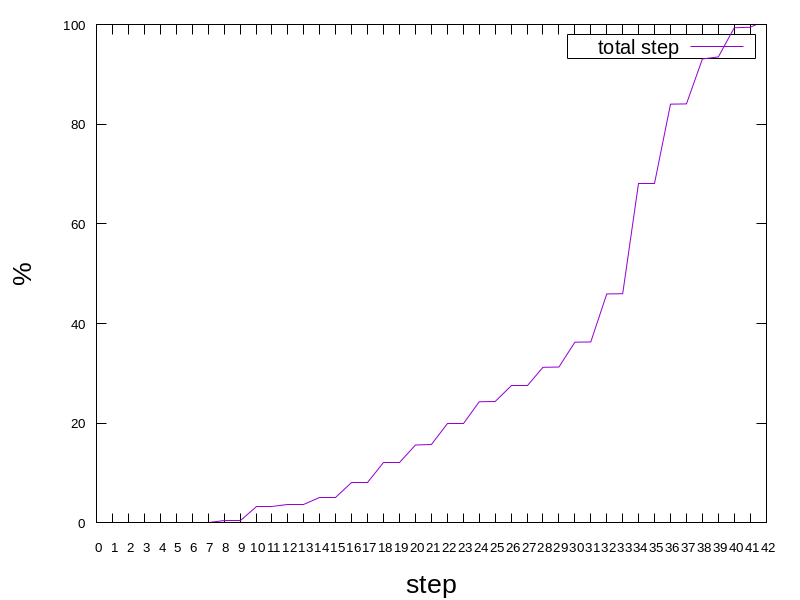
\includegraphics[width=\linewidth]{./figure/stepCum.png}
	\caption{終了手数の分布}
	\label{fig:stepCum}
\end{figure}
\section{評価指標の詳細}

\subsection{group count}
fcountはfatal groupの精度を示す2値(0または1)の指標である.
\begin{equation}
	{C_g = 1 \quad \textrm{If} \quad F_g \cap R_g \ne \phi \quad \textrm{Else} \quad 0}
\end{equation}
例外として$R_g=\phi$(引き分け)の場合,$F_g$も空集合であるならばgroup countは1となる.
\subsection{stone count}
stone countはfatal stoneの精度を示す.stone countの値域は[0, 1]である.
(Count()は集合の要素数を数える関数)
\begin{equation}
	{\textrm{stone count} = \textrm{min}(\frac{\textrm{Count}(F_s \cap R_s)}{4}, 1)  }
\end{equation}
例外として$R_s=\phi$(引き分け)の場合,$F_s$も空集合であるならばstone countは1となる.
\section{データ実験における提案指標の計測}

\begin{enumerate}
	\item 比較手法: 決定木の走査によりたどり着いた$F_s, F_g$によってstone count, group countを計算した
	\item 提案手法: 第3章で述べたアルゴリズムによって収集された最終状態の集合$S=\{s_{edge_1}, s_{edge_2}, ..., s_{edge_{k^l}}\}$
	    を指標ごとにグループ化する.
		\begin{itemize}
			\item group count: fatal groupによって$S$をグループ化してできた集合$\{S_{g_1}, S_{g_2}, ..., S_{g_n}\}$($S_{g_i}$は組み合わせ$g_i$がfatal groupとなっている盤面の集合)
			を要素が多い順に2つ取り出す.抽出された2つの集合$\{S_{g_{m_1}}, S_{g_{m_2}}\}$における$\{g_{m_1}, g_{m_2}\}$で構成される集合を$F_g$とし,group countを計算した.
			\item stone count: $g_{m_1}$を$F_s$とし,stone countを計算した.
		\end{itemize}
		
\end{enumerate}

\section{データ実験に使用したモデルの詳細}
第4章に記載した表\ref{table:result-online}の結果を求める際に用いたモデルのパラメータを表\ref{table:param-data}に示す.
\begin{table}[H]
	\caption{データ実験:使用モデルのパラメータ}
	\centering
	\scalebox{0.98}[0.98]{
		\begin{tabular}{c|c}
			パラメータ名 & 値 \\ \hline
			time    & 対戦時の後番のモデルと同じ \\ 
			$C_{puct}$    & 対戦時の後番のモデルと同じ \\
			エポック数 & 200 \\
			$k$ (提案手法のみ)     & 4 \\
			$l$ (提案手法のみ)     & 2 \\
		\end{tabular}
	}
	\label{table:param-data}
\end{table}

表\ref{table:param-data}の通り,対戦データが生成された際のモデルのパラメータを使用している.
そのため本手法はモデルの構造とパラメータの値へのアクセスが可能な場合を想定したホワイトボックス的アプローチの実験であると言える.
モデルのtime, $C_{puct}$の値を固定して同様の手法を適用した場合の実験結果を\ref{sec:gray}で示す.
\section{末尾のグループ化}
提案手法は予想図とその予想図に至る分岐(両方を合わせて進行図と記載)を抽出する.
図\ref{fig:regroup}は分岐を末尾の3手で2つのグループに再編する様子を表している.(ここでは分岐は行動$a$の連続として表している)
\begin{figure}[t]
	\centering
	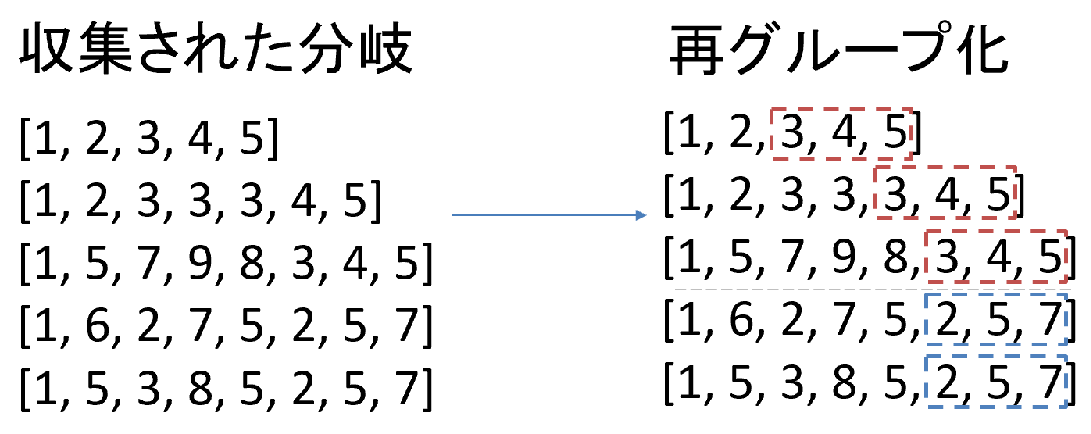
\includegraphics[width=\linewidth]{./figure/regroup.pdf}
	\caption{再グループ化}
	\label{fig:regroup}
\end{figure}
取り出された分岐を末尾の3手の選択でさらにグループ化した結果,元の分岐の数と再グループ化された分岐の数の平均は
表\ref{table:tail}のようになった.
結果として,取り出された分岐のうち,平均約2$\sim$3つの分岐において末尾の3手が共通する傾向にあることがわかった.
\begin{table}[H]
	\caption{再グループ化した際の分岐の数}
    \scriptsize
    \label{table:tail}
	\centering
	\scalebox{0.98}[0.98]{
		\begin{tabular}{c|c|c||c}
			手数(盤面数, 補間の有無)&  再グループ化前の分岐数(平均)&  再グループ化後の分岐数(平均)\\ \hline
			19-24(9862, 無)    & 7.01 & 3.00  \\
			19-24(9862, 有)    & 13.62 & 4.43  \\
			13-24(21022, 無)   &  & 3.08  \\
			13-24(21022, 有)   &  & 4.51 \\
		    0-40(61021,無)& 5.23 & 2.23\\
		    0-40(61021,有)& 10.82 & 3.78\\
		\end{tabular}
	}

	
\end{table}
また,各分岐の長さの平均は\ref{fig:length}のようになった.
尚,正確には1つの盤面,行動(最も訪問回数が大きい行動)の組に対して取り出される軌道の平均を更に平均した値を示している.
\begin{table}[H]
	\caption{分岐の長さの平均}
    \scriptsize
    \label{fig:length}
	\centering
	\scalebox{0.98}[0.98]{
		\begin{tabular}{c|c}
			手数(盤面数, 補間の有無)&  分岐の長さ(平均)\\ \hline
		    0-40(61021,無)& 10.89\\
		    0-40(61021,有)& 15.31\\
		\end{tabular}
	}	
\end{table}

\section{グレーボックス的手法}
\label{sec:gray}
モデルのパラメータを固定し,再び第4章のデータ実験を行った.パラメータの値を固定しているため,本実験はモデルの具体的なパラメータの値へのアクセスが不可能な場合にも適用可能な
グレーボックス的手法であると言える.
固定されたパラメータを表\ref{table:param-data-extra}に示す.
\begin{table}[H]
	\caption{データ実験(追加):使用モデルのパラメータ}
	\centering
	\scalebox{0.98}[0.98]{
		\begin{tabular}{c|c}
			パラメータ名 & 値 \\ \hline
			time    & 5 \\ 
			$C_{puct}$    & 1 \\
			エポック数 & 200 \\
			$k$ (提案手法のみ)     & 4 \\
			$l$ (提案手法のみ)     & 2 \\
		\end{tabular}
	}
	\label{table:param-data-extra}
\end{table}

実験の結果は表\ref{table:result-offline}のようになった.第4章に記載したホワイトボックス的手法と同様に提案手法はgroup countにおいて比較手法より高い値を示した.
\begin{table}[H]
	\caption{実験結果:データ実験}
	\centering
	\scalebox{0.98}[0.98]{
		\begin{tabular}{c|c|c|c|c}
			\multicolumn{1}{c}{} & \multicolumn{2}{|c|}{group count} 
			& \multicolumn{2}{c|}{stone count}\\ \hline \hline
			手数(盤面数, 補間の有無)    & 提案手法 & 比較手法 & 提案手法 & 比較手法 \\ \hline
			19-24(9862, 無)    & \bf{0.60} & 0.44 & 0.61 & \bf{0.63} \\
			19-24(9862, 有)    & \bf{0.63} & 0.44 & 0.61 & \bf{0.63}  \\
			13-24(21022, 無)   & \bf{0.53} & 0.37 & 0.55 & \bf{0.56}  \\
			13-24(21022, 有)   & \bf{0.55} & 0.37 & 0.55 & \bf{0.56}  \\
		\end{tabular}
	}
	\label{table:result-offline}
\end{table}
